\section{NP complete problems}
% Definitions
\begin{itemize}
	\item \textbf{Kompleksitetsklassen} $\mathbf P$ er klassen af sprog, der kan blive besluttet i polynomiel tid af en Turing maskine
	\item \textbf{NP} er klassen af sprog $L$ hvor der eksister et sprog $L' \in \mathbf P$ og et polynomium $p$ således at
  \begin{equation*}
    \forall v: x \in L \Leftrightarrow [\exists y \in \{0,1\}^* : |y| \leq p(|x|) \land \langle x, y \rangle \in L']
  \end{equation*}
  \item Given to sprog $L_1$ og $L_2$ reducerer $L_1$ til $L_2$, hvis der er en polynomiel udregnelig funktion $r$ således at for alle $x \in \{0,1\}^*$ har at
  \begin{equation*}
    x \in L_1 \Leftrightarrow x \in L_2
  \end{equation*}
  Skrevet som $L_1 \leq L_2$ 
  \item Et sprog $L$ er et $\mathbf{NP}$ hård sprog, hvis den har den egenskab af for alle $L' \in \mathbf{NP}$, $L'$ reducerer til $L$ 
  \item Klassen $\mathbf{NPC}$ er klassen af $\mathbf{NP}$ komplette sprog, som er de sprog i $\mathbf{NP}$ som er $\mathbf{NP}$ hårde.
\end{itemize}

\subsection{SAT og varianter af SAT}
\begin{itemize}
  \item The \textbf{Satisfiability Problem} (SAT) er følgende decision problem: Given en CNF formula, afgør hvorvidt der er en assignment af sandhed værdier til variablerne der gør at formulaen evaluere til sand
  \item \textbf{Cook's Theorem} $\text{SAT} \in \mathbf{NPC}$
  \item Lad $k$ SAT, hvor $k \geq 1$ er en integer, være den situation af SAT hvor formelen er på CNF form og alle clases har $k$ literals 
  \item \textbf{Proposition} 3SAT er $\mathbf{NP}$ komplet 
  \begin{itemize}
  	\item Dette følger af reduktionen fra CIRCUIT SAT til SAT, siden den ikke bruger mere en 3 literals
  \end{itemize} 
  \item \textbf{Collary} 2SAT er i $\mathbf{NL}$ hvilket er en delmængde af $\mathbf{P}$ 
  \begin{itemize}
  	\item $\mathbf{NL}$ er kompleksitetsklassen, som kan blive løst med en logaritmisk mængde af plads
  \end{itemize}
  \item NAESAT er det problem hvor der er ingen clauses hvor alle træ literals er lig hinanden 
  \item \textbf{Theorem} NAESAT er $\mathbf{NP}$ komplet
  \begin{proof} 
    For at bevise at NAESAT er $\mathbf{NP}$ komplet kan man lave en reduktion fra CIRCUIT SAT til NAESAT. Samme reduktion bruges som til SAT, hvor der tilføjes en variable $z$ til alle clauses af længde $1$. Dette er en korrekt reduktion siden alle af størrelse 2 og 3 aldrig alle sammen kan være sande i en satisfying assignment. Hvis NAESAT sætter $z$ til sand er den negeret version også satisfying assignment og derfor er der også en satisfying assignment assignment til CIRCUIT SAT
  \end{proof}
\end{itemize}

\subsection{Graf problemer}
\begin{itemize}
  \item 3 COLORING er følgende problem: Given en undirected graf $G=(V,E)$ find en farvelægning af knuderne $V$ således at ingen kanter $ij \in E$ eksistere således at $i$ og $j$ har samme farve.
	\item \textbf{Theorem} 3 COLORING is $\mathbf{NP}$ komplet  
  \item For en undirected graf $G=(V,E)$ lad $I \subseteq V$ 
  \begin{itemize}
  	\item $I$ er \textbf{uafhængig} hvis for $i,j \in I$, $ij \notin E$
  \end{itemize}
  \item INDEPENDENT SET problemet er følgende: Givet en undirected graf $G=(V,E)$ og et mål $k$ er der et independent set $I$ hvor $|I| = K$ 
  \item \textbf{Theorem} INDEPENDENT SET er $\mathbf{NP}$ komplet
  \begin{proof} 
    \begin{figure}[ht]
    	\centering
    	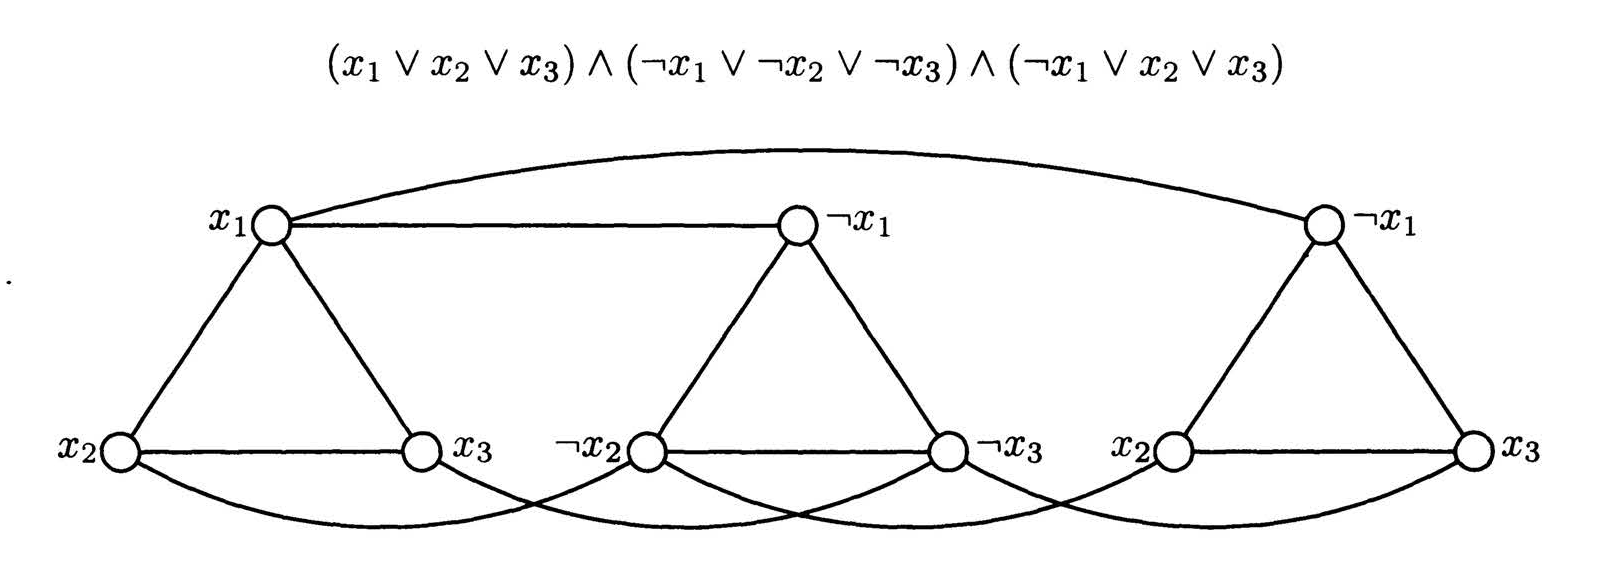
\includegraphics[width=\linewidth]{img/independent}
    	\caption{Reduktion til INDEPENDENT SET\label{label}}
    \end{figure}
    Reduktionen er fra 3SAT, hvor vi har formelen $\phi$ i CNF form med variabler $x_1, \dots, x_n$ og clauses $C_1, \dots, C_m$. Beviset bruger en trekant gadget for hver clause, hvor hver knude representere en literal. En trekant gadget nemlig den egenskab, at dens største independent set har størrelse $1$. Derfor kan den bruges til at vælge hvilken literal skal være sand. For at sikre sig at variablerne er konsistente har hver variabel en kant til alle dens negationer i de andre clauses for at sikre sig at de ikke begge to kan være korrekt. Der eksisterer dermed en satisfying assignment, hvis den resulterende graf har et independent set med størrelse $n$. Denne reduktion er polynomiel siden den kun behøves kigge på hver clause en gang og hver variabel $n$ gange, hvor $n$ er antallet af variabler og per tideligere argumentationer er den korrekt. 

  \end{proof}
  \item CLIQUE problemet er følgende: Given en undirected graf $G$ og et mål $K$ eksitere der et set af $K$ knuder der har mulige kanter mellem dem
  \item NODE COVER problemet er følgende: Given en undirected graf $G$ er der et set $C$ med $B$ eller mindre således af hver edge i $G$ har mindst en af den endpoints i $C$ 
  \item \textbf{Corollary} CLIQUE og NODE COVER er $\mathbf{NP}$ komplet 
  \begin{itemize}
  	\item Dette følger af at CLIQUE er den inverse af INDEPENDENT SET og at hvis $I$ er et independent set hvis og kun hvis $V-I$ er et node cover af den samme graf.
  \end{itemize}
  \item HAMILTON PATH problemet er følgende problem: Givet en undirected graf $G$ har den en Hamilton path dvs. en path hvor den besøger hver knude præcis en gang
  \item \textbf{Theorem} HAMILITON PATH er $\mathbf{NP}$ komplet
  \begin{proof} 
  \begin{figure}[ht]
  	\centering
  	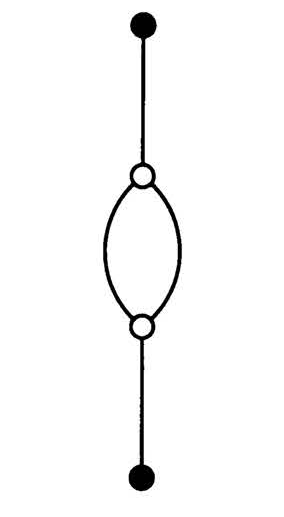
\includegraphics[width=70px]{img/choice_gadget}
  	\caption{Choice gadget\label{fig:choice}}
  \end{figure}

  \begin{figure}[ht]
  	\centering
  	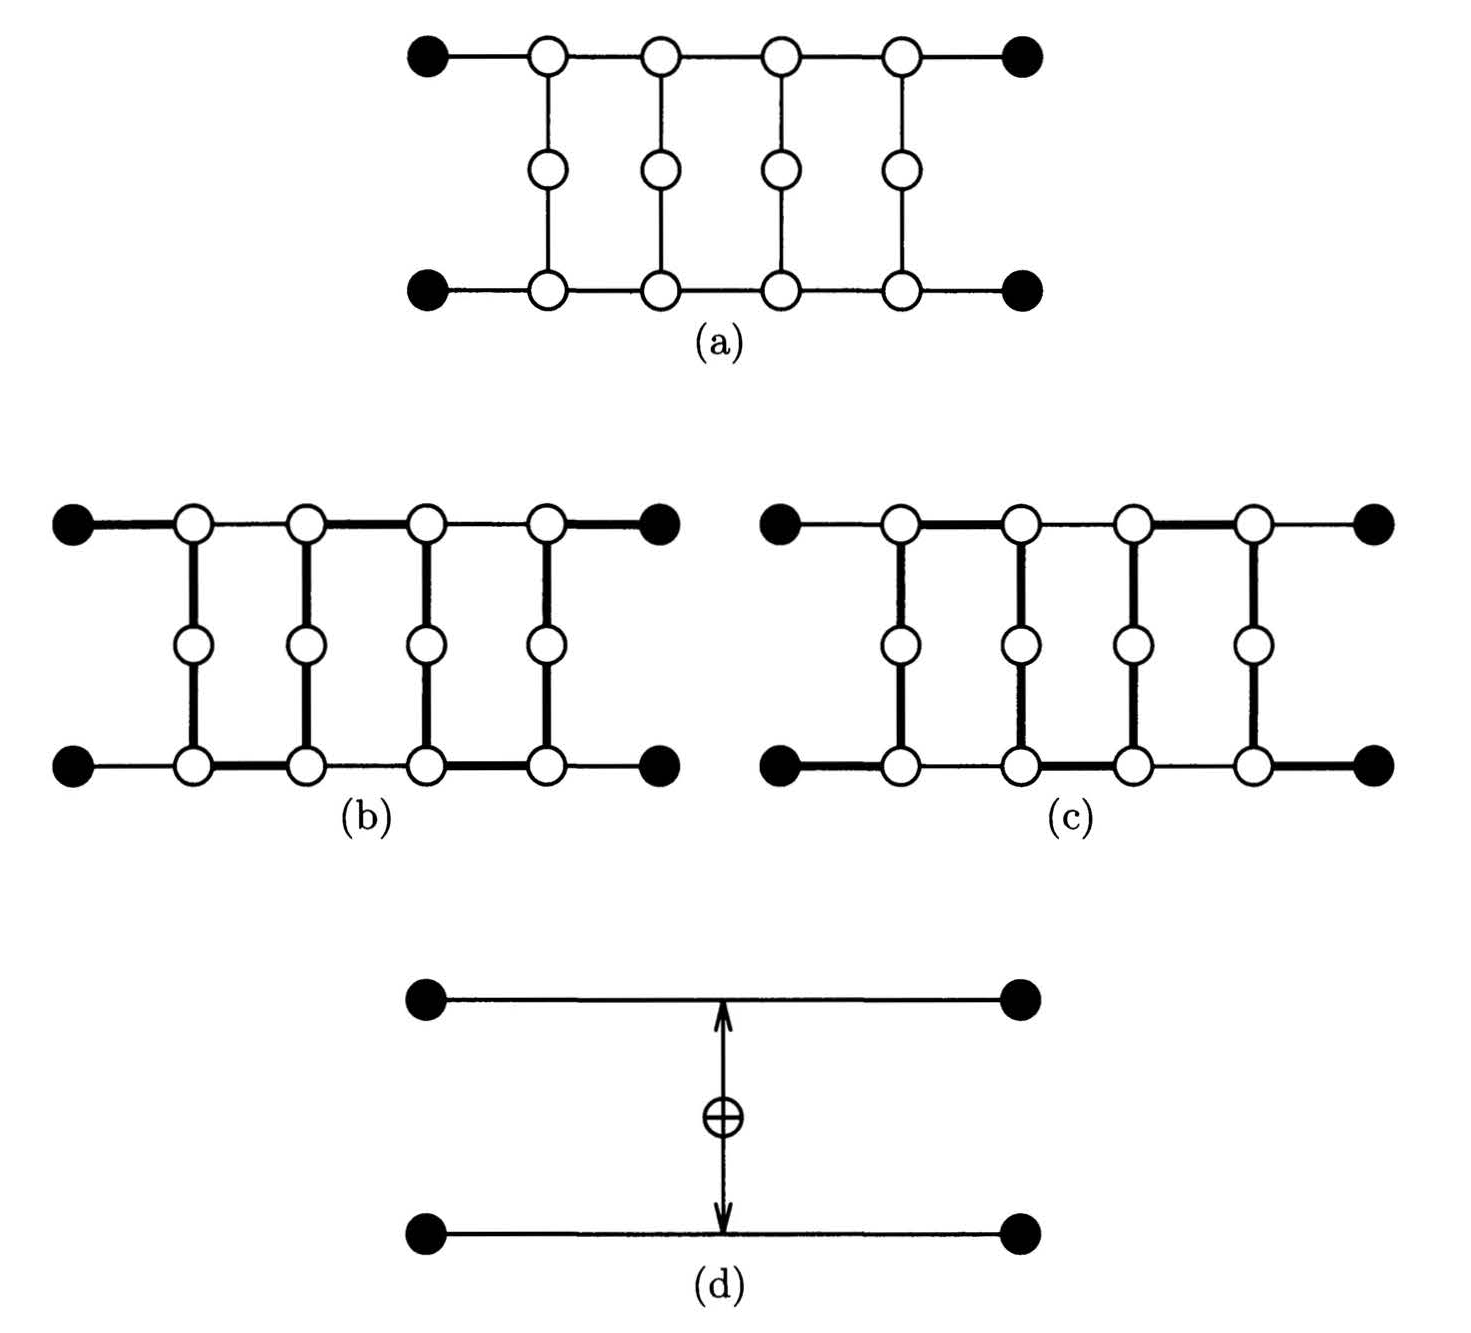
\includegraphics[width=350px]{img/consistency_gadget}
  	\caption{Consistency gadget\label{fig:consistency}}
  \end{figure}

  \begin{figure}[ht]
  	\centering
  	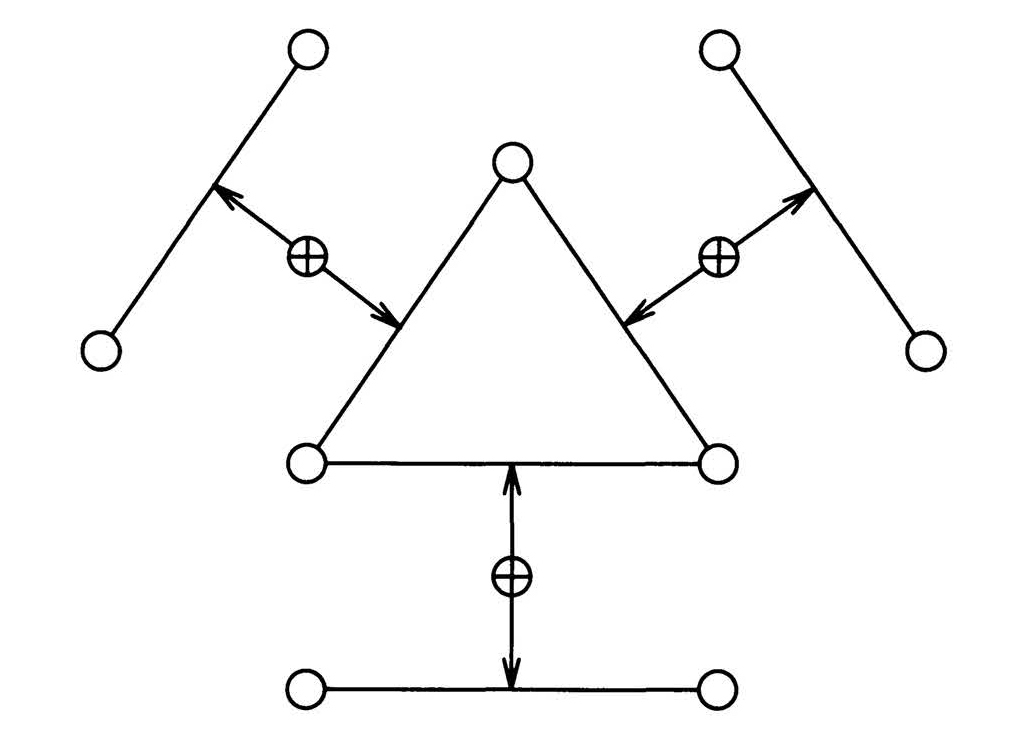
\includegraphics[width=300px]{img/constraint_gadget}
  	\caption{Constraint gadget\label{fig:constraint}}
  \end{figure}


    Reduktionen er fra 3SAT, hvor vi har formelen $\phi$ i CNF form med variabler $x_1, \dots, x_n$ og clauses $C_1, \dots, C_m$. Der bliver konstrueret en graf $R(\phi)$ således, at den har en Hamilton path hvis og kun hvis $\phi$ er satisfiable. Et choice gadget (Figur \ref{fig:choice}) bliver brugt til at vælge mellem sandhedsværdier for de individuelle variabler. For at sikre sig grafen er konsistent bruges en consistency gadget (Figur \ref{fig:consistency}(a)), den har den egenskab at man kun kan traverse en af kanterne (vist på (b) og (c)). Derfor er det også kaldet en xor gate. For hver clause bruges en constraint gadget (Figur \ref{fig:constraint}) til at vælge hvilken af variablerne der skal være sand. Den af siderne der ikke bliver traversed vælges til at være korrekt. Xor gadgets bliver brugt til at sørge for consistency med choice gadgets. Ud fra det laves en graf, hvor man starter i en knude med en kant til den første choice gadget. Dernæst er alle choice gadgets chained sammen hvori den sidste ender ud i en knude, som har kanter til alle knuder i trekanterne og har en kant til en knude som ikke har andre kanter. Et eksempel kan ses i Figur \ref{fig:hamil-example} \smallskip 
  
    Grunden til at denne reduktion virker er: \\
    Hvis der eksisterer en satisfying assignment til $\phi$, må det gælde at den satisfying assignment er en Hamilton path siden, at mindst en i hver er clause er sand og derfor er det muligt at lave en Hamilton path. \\
    Hvis der eksisterer en Hamilton path, kan man finde en satisfying assignment ved at bruge assignments fra choice gadgets. Grunden til at den er satisfying er, at vi ved der er mindst en af hver literals i hver clause er sand. Derfor må reduktionen være korrekt. Hamilton path er i NP og derfor er den NP komplet. 

  \end{proof}
  \item \textbf{Corollary} TSP er $\mathbf{NP}$ komplet
  \begin{proof} 
    TSP reduceres til HAMILTON PATH: Given en graf $G$ med $n$ knuder, defineres en distance matrix $d_{ij}$ og en budget $B$ således at der kun er en Hamilton path i den original graf hvis og kun hvis der er en tour med længde $B$ eller mindre. Der er $n$ byer en fra hver knude i grafen. Distancen mellem to byer $i$ og $j$ er $1$ hvis der er en kant $ij$ i grafen og $2$ ellers. Budget sættes til $B=n+1$ 

  \end{proof}
\end{itemize}

\subsection{Mængder og tal}
\begin{itemize}
  \item TRIPARTITE MATCHING er følgende problem: Givet træ mængde $B$, $G$, $H$, hvor alle træ har størrelse $n$, og en relation $T \subseteq B \times G \times H$. 
  \item \textbf{Theorem} TRIPARTITE MATCHING er $\mathbf{NP}$ komplet
  \item KNAPSACK er følgende problem: Man skal vælger mellem et set af $n$ objekter. Objekt $i$ har værdi $v_i$ og vægt $w_i$, hvor om det gælder at $v_i, w_i \geq 0$. Der er en grænse $W$ på hvor meget man må vælge. Man skal finde et subset $S \subseteq \{1,\dots,n\}$ således at $\sum_{i \in S} w_i \leq W$ og $\sum_{i \in S v_i} v_i \geq K$, hvor $K$ er målet. 
  \item \textbf{Theorem} KNAPSACK er $\mathbf{NP}$ komplet
  \item BIN PACKING er følgende problem: Givet $N$ positive integers $a_1, a_2, \dots, a_N$ (objekterne), kapaciteten $C$ og antallet af bins $B$. Problemet er så hvorvidt disse tal kan blive in delt i $B$ subset, hvor hver af summerne højest giver $C$ 
  \item \textbf{Theorem} BIN PACKING er $\mathbf{NP}$ komplet
\end{itemize}

\begin{figure}[H]
  \centering
  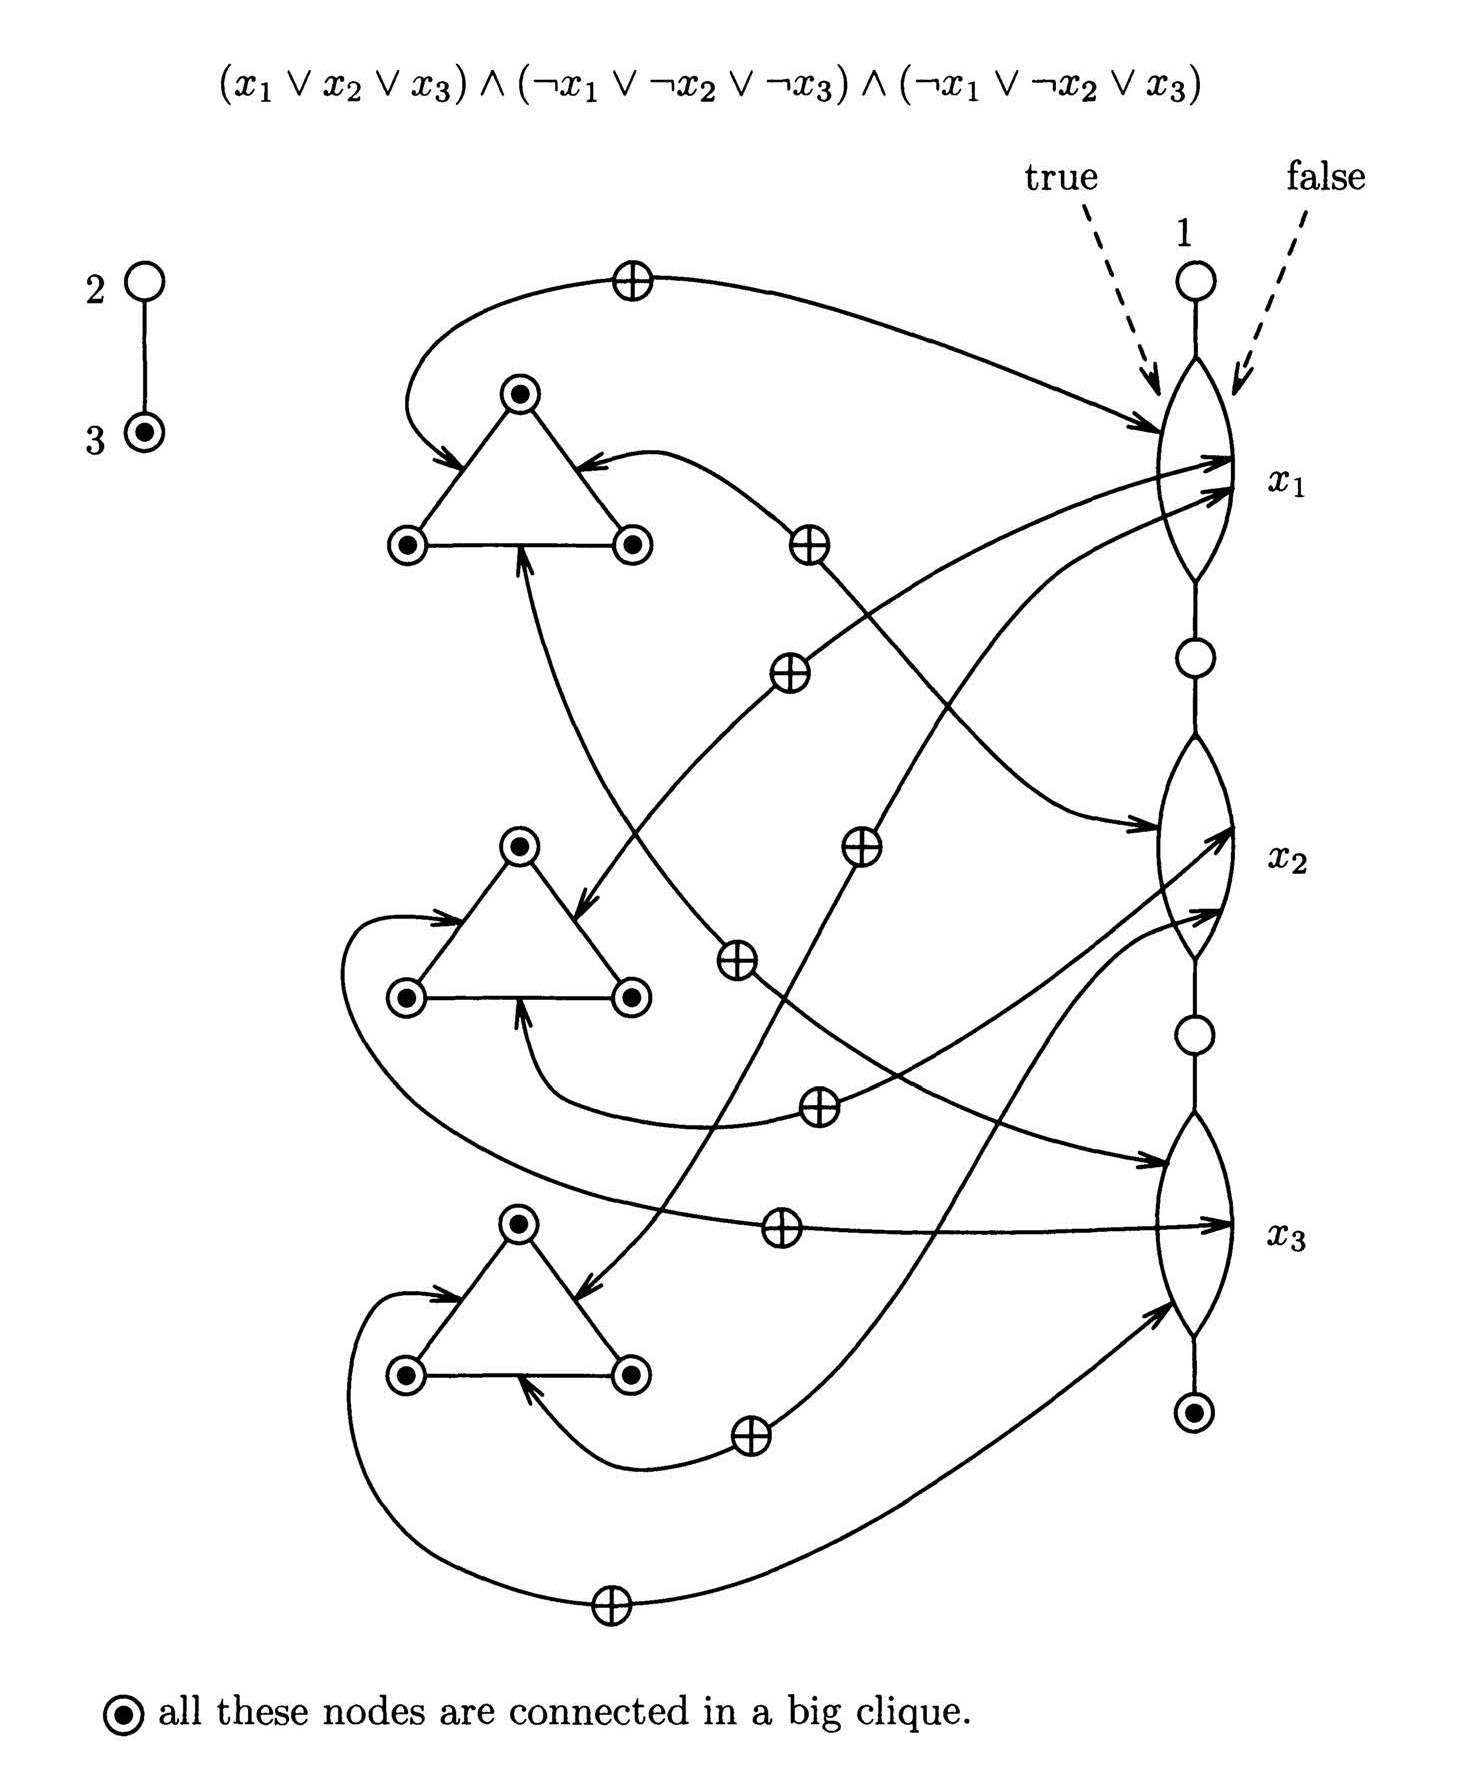
\includegraphics[width=\linewidth]{img/hamil_example}
  \caption{Reduktion fra 3SAT til HAMILTON PATH\label{fig:hamil-example}}
\end{figure}

\newpage
%%% Local Variables:
%%% mode: latex
%%% TeX-master: "optimering-noter"
%%% End:
